\begin{frame}\frametitle{Measurement Goal}
  \scriptsize
  Total ($\sigma$) and the differential ($\frac{d\sigma}{dP_T^{\gamma}}$) cross sections of $W\gamma\rightarrow l\nu\gamma$.\\
  $\sigma = \frac{N}{L}$, $\frac{d\sigma}{dP_T^{\gamma}} = \frac{N}{L \Delta P_T^{\gamma}}$, \\
  \tiny
  where $N$ is a number of $W\gamma$ events produced during a given period of time, $L$ is an integrated LHC luminocity during the same period of time, $\Delta P_T^{\gamma}$ is a $P_T^{\gamma}$ bin width.
  \scriptsize
  - - - - - - - - - - - - - - - \\
  Phase space definition:
  \begin{itemize}
    \scriptsize
    \item $P_T^{\gamma}>$ 15 GeV;
    \item $\Delta{R}(\gamma,lep) > $0.7;
    \item several more requirements related to geometric and kinematic limitations
  \end{itemize}
  - - - - - - - - - - - - - - - \\
  \tiny
  Notations:
  \begin{itemize}
    \tiny
    \item Transverse momentum ($P_T$):  a photon momentum component transverse to the proton beamline
    \item Cone separation: $\Delta R(a,b) = \sqrt( (\phi_a-\phi_b)^2 + (\eta_a-\eta_b)^2 )$;
    \item Pseudorapidity: $\eta=-ln \left[ tan{(\theta/2)} \right]$
    \item EB and EE: ECal barrel and ECal endcap
  \end{itemize}
\begin{figure}[htb]
  \begin{center}
    {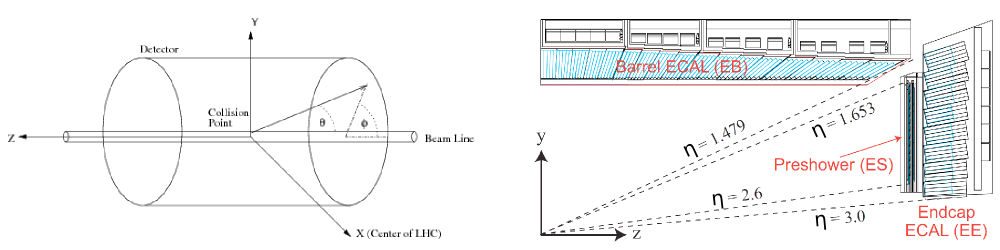
\includegraphics[width=0.90\textwidth]{../figs/ForPresentation/CMS_coordSyst_and_ECal.png}}
  \end{center}
\end{figure}
\end{frame}%{Measurement Goal}

\begin{frame}\frametitle{Measurement Strategy}
  \scriptsize

$\sigma = \frac{N}{L}~\rightarrow~\sigma = \frac{N_{sel}-N_{bkg}}{A \epsilon L}$ 

$\frac{d\sigma}{dP_T^{\gamma}} = \frac{N}{L \Delta P_T^{\gamma}}~\rightarrow~\frac{N_{sel}^i-N_{bkg}^{i}}{(A\epsilon)^i L \Delta P_T^{\gamma}^i}$

\begin{table}[h]
  \scriptsize
  \begin{center}
  \begin{tabular}{|l|c|c|}
    \hline
          & \multicolumn{2}{|c|}{Algebraic representation for} \\ 
     Step & \multicolumn{2}{|c|}{the measurement of} \\ 
          & $d\sigma/dP_{T}^{\gamma}$ & $\sigma$ \\ \hline
    select events & {\bfseries{$N_{sel}^i$}} &    {\bfseries{$N_{sel}$}}       \\ \hline
    subtract background & {\bfseries{$N_{sign}^i = N_{sel}^i - N_{bkg}^i$}} &    {\bfseries{$N_{sign}=N_{sel}-N_{bkg}$}}       \\ \hline
    correct for eff X acc & $N_{ph.sp.}^i = \frac{N_{sign}^i}{(A \times\epsilon)^i}$ &  $N_{ph.sp.}=\frac{N_{sign}}{A\times\epsilon}$       \\ \hline
    compute cross section & $ \left( \frac{d\sigma}{dP_{T}^\gamma} \right) ^i = \frac{N_{ph.sp.}^i}{L \cdot (\Delta P_T^\gamma)^i}$  &  $\sigma = N_{ph.sp.}/L$       \\ \hline
    \multicolumn{3}{|l|}{estimate systematic uncertainties}          \\ \hline
  \end{tabular}
  \label{tab:analysisOutline}
  \end{center}
\end{table}
\end{frame}%{Measurement Strategy}
